\subsection{Detektorspannung in Abh�ngigkeit der Chopperfrequenz}
\label{sec:chopper}
Zuerst soll der Zusammenhang zwischen der Detektorspannung U und der Chopperfrequenz f untersucht werden. Die Chopperfrequenz wird im Bereich von 10Hz bis 50Hz variiert. Bei Werten unter 10Hz ist die Schwankung der Werte zu gro�, so dass die Signale nicht vom Untergrund unterschieden werden k�nnen. Die Detektorspannung wird am Lock-In-Verst�rker abgelesen. Es wurde ein Fehler von 40-10 mV angenommen, je nach Schwankung der Nadel. Der Plot der Messdaten mit linearen Achsen ist in Abbildung \ref{fig:chopper_lin} zu sehen. In Abbildung \ref{fig:chopper_log} sind die Messdaten mit doppelt logarithmischen Achsen geplottet. Da ein linearer Zusammenhang zwischen log(U) und log(f) zu sehen ist, werden die Messdaten mit  Gleichung \ref{eqn:chopperfit} gefittet. Die Messdaten f�r den Fit befinden sich im Anhang, in Tabelle \ref{tab:chopper}.

\begin{align}
\label{eqn:chopperfit}
U(f) = \exp[A \cdot \log(f) + B]
\end{align}

Dabei sind A und B freie Parameter, die durch den Fit bestimmt werden. Das Ergebnis des Fits ist in Tabelle \ref{tab:chopperfit} zu sehen.

\begin{figure}[H]
\centering
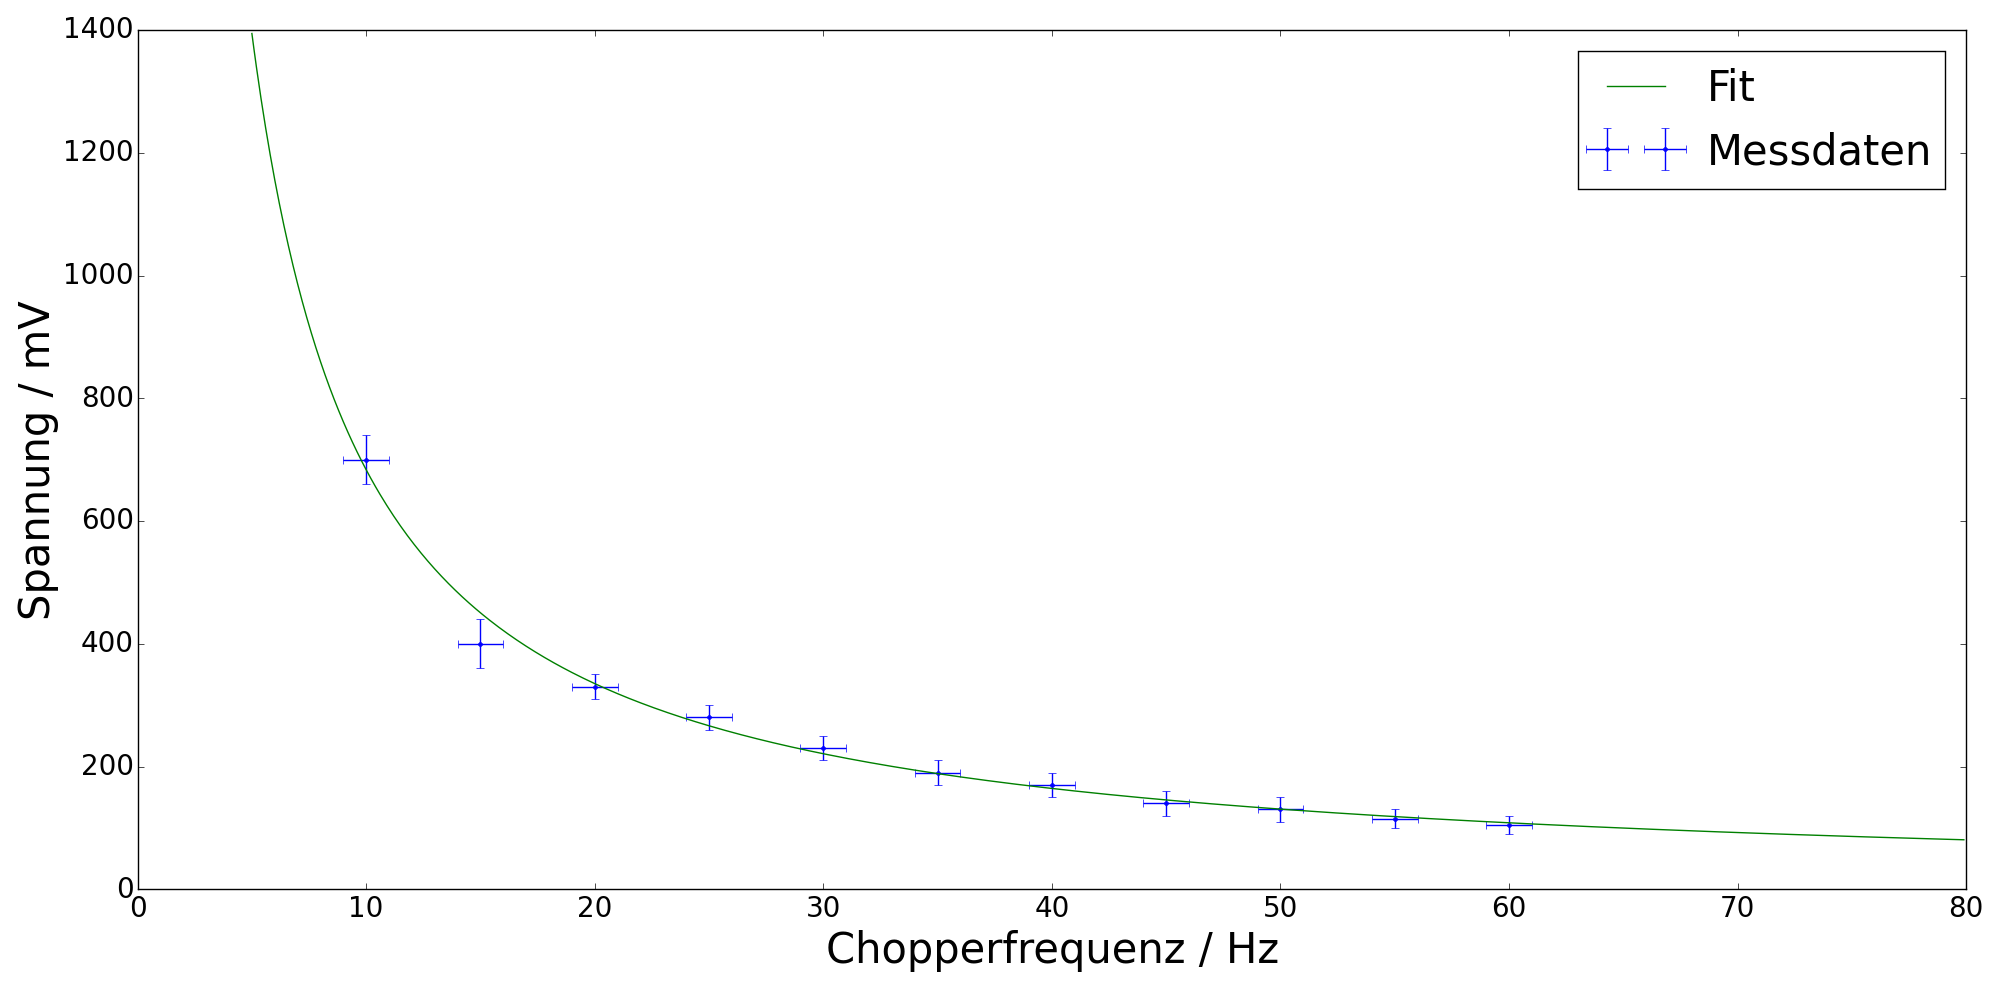
\includegraphics[scale = 0.33]{chopper_lin.png}
\caption{Spannung in Abh�ngigkeit der Chopperfrequenz mit linearen Achsen}
\label{fig:chopper_lin}
\end{figure}

\begin{figure}[H]
\centering
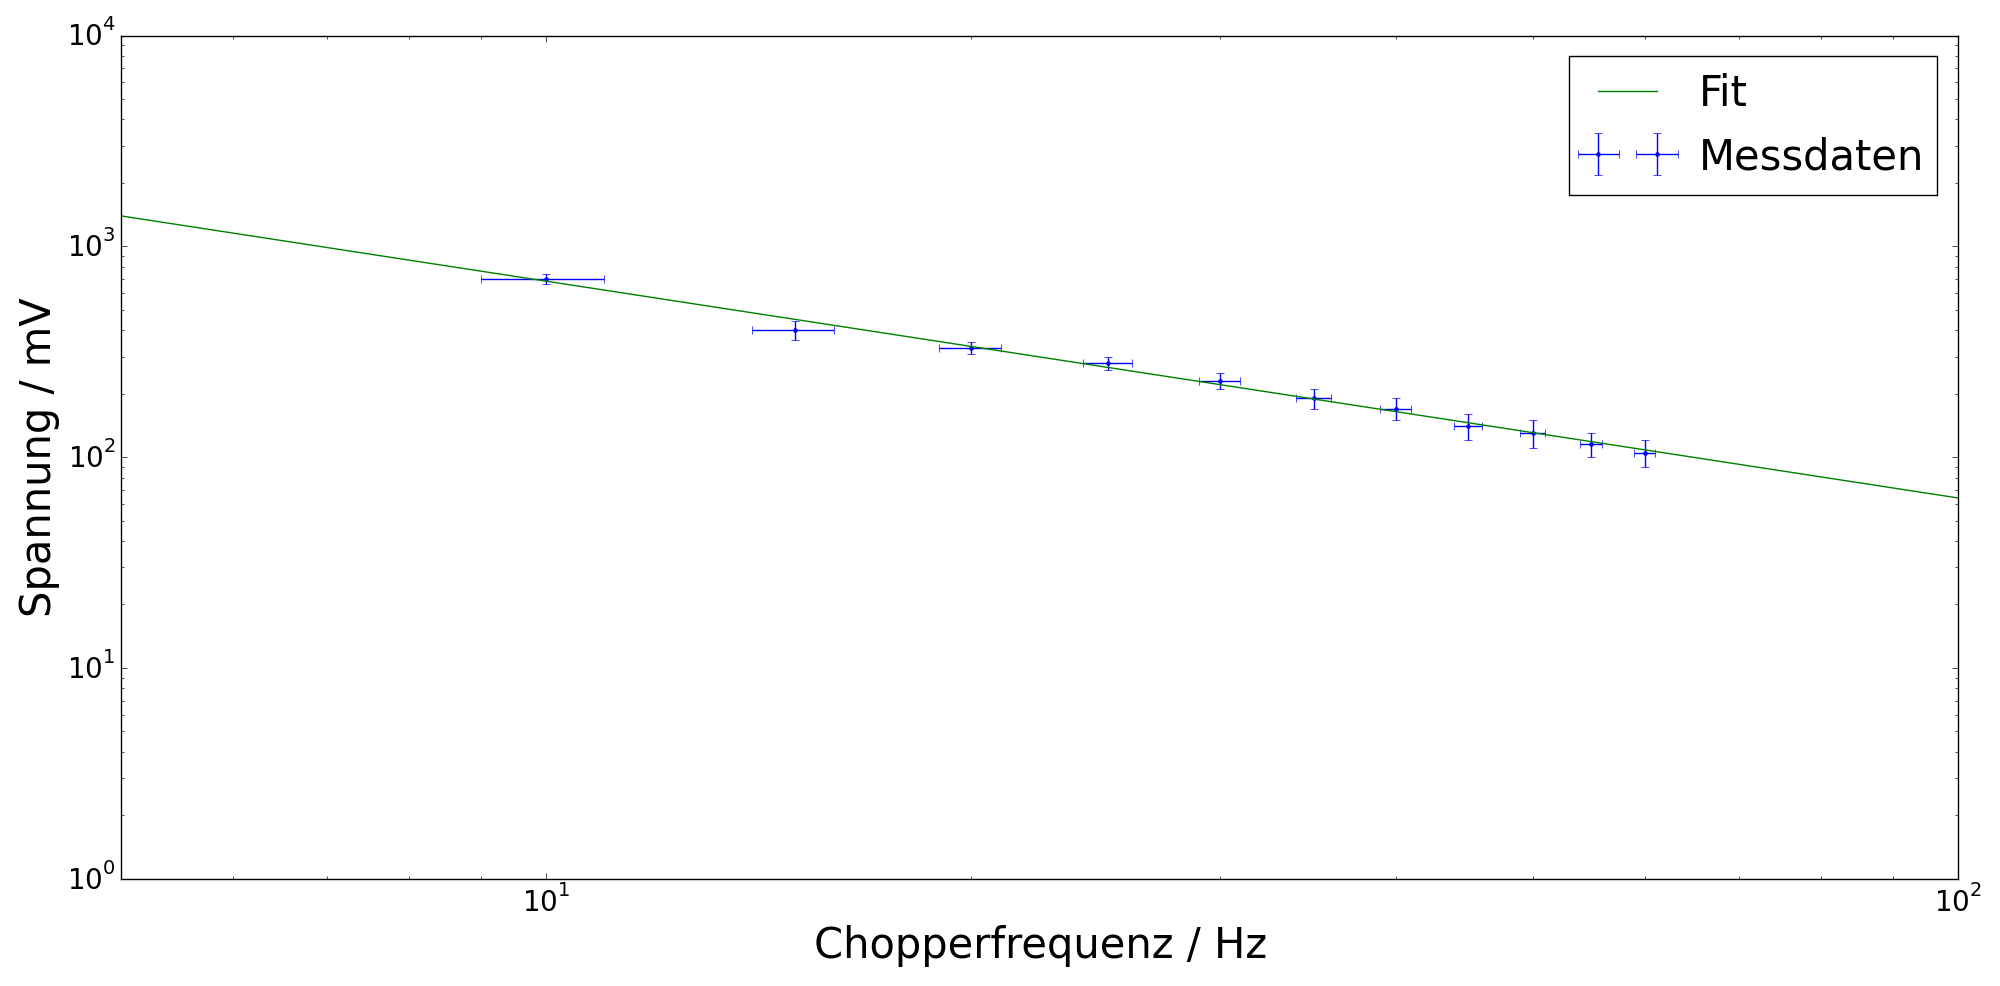
\includegraphics[scale = 0.33]{chopper_log.png}
\caption{Spannung in Abh�ngigkeit der Chopperfrequenz mit logarithmischen Achsen}
\label{fig:chopper_log}
\end{figure}

\begin{table}[H]
\caption{Fitparameter f�r den Fit der Spannung in Abh�ngigkeit der Chopperfrequenz nach Gleichung \ref{eqn:chopperfit}}
\label{tab:chopperfit}
\centering
\begin{tabular}{|c|c|}
\hline Parameter & Wert \\ 
\hline A & -1,03(3) \\ 
\hline B & 8,89(8) \\ 
\hline $\chi_{red}^2$ & 1,22 \\ 
\hline 
\end{tabular} 
\end{table}

Das $\chi_{red}^2$ von 1,22 spricht daf�r, das der Zusammenhang zwischen der Chopperfrequenz und der Spannung gut durch das Modell beschrieben wird. Bei kleinen Frequenzen erreicht der Detektor eine S�ttigung. Aus dem Parameter A folgt, dass die Spannung proportional zu 1/f ist. F�r den folgenden Versuchsteil wird eine Chopperfrequenz von 30Hz verwendet.
